\documentclass[11pt]{article}
\usepackage{
    amsmath, 
    amssymb, 
    amsthm, 
    graphicx, 
    geometry, 
    listings, 
    xcolor, 
    url, 
    enumitem, 
    fancyhdr, 
    multirow, 
    caption
}
\geometry{margin=1in}
\definecolor{darkgreen}{rgb}{0,0.5,0}
\pagestyle{fancy}

\lhead{SFSU, CSC 645-01}
\chead{Spring 2025}
\rhead{Computer Networks}

\title{Homework 3}
\author{Bryan Lee\\922649673}
\date{May 4, 2025}

\begin{document}

\maketitle
\thispagestyle{fancy}

\section*{Questions}

% Answer variables
\newcommand{\answerOne}{\textbf{
    \begin{enumerate}
        \item Forwarding: The router-local action of transferring a packet from an input link interface to the appropriate output link interface. 
        It typically takes place at very short timescales (typically a few nanoseconds), and is often implemented in hardware.
        \item Routing: The network-wide process that determines the end-to-end paths that packets take from source to destination.
        It typically takes place on much longer timescales (typically seconds), and is often implemented in software.
    \end{enumerate}
    Aside from differences in scale, timescale, and implementation, 
    the key distinction between the two functions is that routing determines the path a packet should take through the network, 
    while forwarding carries out that path by directing the packet to its next hop at each router.
}}

\newcommand{\answerTwo}{\textbf{
    \begin{table}[h!]
        \centering
        \renewcommand{\arraystretch}{1.5}
        \begin{tabular}{|c|c|c|}
            \hline
            \textbf{Subnet Location} & \textbf{IP address of the subnets} \\
            \hline
            Upper LAN (3 hosts) & 223.1.1.0/24 \\
            \hline
            Link b/w top and left router & 223.1.9.0/24 \\
            \hline
            Link b/w top and right router & 223.1.7.0/24 \\
            \hline
            Link b/w left and right router & 223.1.8.0/24 \\
            \hline
            Lower Left LAN (2 hosts) & 223.1.2.0/24 \\
            \hline
            Lower Right LAN (2 hosts) & 223.1.3.0/24 \\
            \hline
        \end{tabular}
        \caption{IP address of the subnets in the network diagram}
    \end{table}
    \begin{figure}[ht]
        \centering
        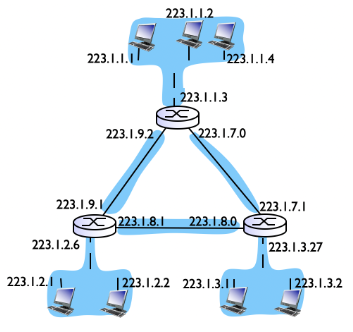
\includegraphics[width=0.5\linewidth]{network-diagram.png}
        \caption{Provided network diagram}
    \end{figure}
}}

\newcommand{\answerThree}{\textbf{
    \begin{table}[h!]
        \centering
        \renewcommand{\arraystretch}{1.5}
        \begin{tabular}{|c|c|c|c|c|c|c|c|}
            \hline
            \textbf{Step} & \textbf{N'} & \textbf{D(y), p(y)} & \textbf{D(v), p(v)} & \textbf{D(w), p(w)}
            & \textbf{D(t), p(t)} & \textbf{D(u), p(u)} & \textbf{D(z), p(z)} \\
            \hline
            0 & x & 6,x & 3,x & 6,x & $\infty$ & $\infty$ & 8,x \\
            \hline
            1 & x,v & 6,x & - & 6,x & 7,v & 6,v & 8,x \\
            \hline
            2 & x,v,y & - & - & 6,x & 7,v & 6,v & 8,x \\
            \hline
            3 & x,v,y,w & - & - & - & 7,v & 6,v & 8,x \\
            \hline
            4 & x,v,y,w,u & - & - & - & 7,v & - & 8,x \\
            \hline
            5 & x,v,y,w,u,t & - & - & - & - & - & 8,x \\
            \hline
            6 & x,v,y,w,u,t,z & - & - & - & - & - & - \\
            \hline
        \end{tabular}
        \caption{Dijkstra's Algorithm Table}
    \end{table}
    \newpage
    \begin{table}[h!]
        \centering
        \renewcommand{\arraystretch}{1.5}
        \begin{tabular}{|c|c|}
            \hline
            \textbf{Destination} & \textbf{Outgoing link} \\
            \hline
            z & (x,z) \\
            \hline
            y & (x,y) \\
            \hline
            w & (x,w) \\
            \hline
            v & (x,v) \\
            \hline
            t & (x,v) \\
            \hline
            u & (x,v) \\
            \hline
        \end{tabular}
        \caption{Forwarding Table}
    \end{table}
    \begin{center}
        z, y, w are directly connected to x. \\
        v, t, u are connected to x via v.
    \end{center}
    \begin{figure}[ht]
        \centering
        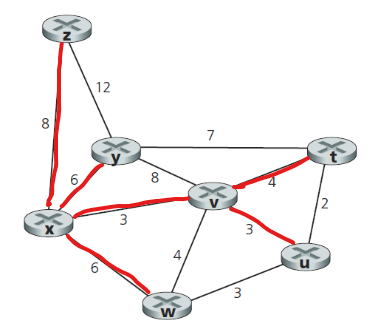
\includegraphics[width=0.5\linewidth]{shortest-path-tree.png}
        \caption{Shortest-path tree from x to all nodes}
    \end{figure}
}}

\newcommand{\answerFour}{\textbf{
    List of IP addresses of the subnets:
    \begin{enumerate}[label=\arabic*.]
        \item Add the cost from C to B to the distance vector from B: \\
            \begin{equation*}
                (5+6, 0+6, 8+6, 3+6, 6+6, 2+6) = 
                (11, 6, 14, 9, 12, 8)
            \end{equation*}
        \item Add the cost from C to D to the distance vector from D:
            \begin{equation*}
                (6+3, 7+3, 6+3, 0+3, 9+3, 10+3) = 
                (9, 10, 9, 3, 12, 13)
            \end{equation*}
        \item Add the cost from C to E to the distance vector from E:
            \begin{equation*}
                (7+5, 6+5, 3+5, 2+5, 0+5, 4+5) = 
                (12, 11, 8, 7, 5, 9)
            \end{equation*}
        \item Finding the distance among the paths via B, D, and E:
            \begin{itemize}
                \item To A: min(11, 9, 12) = 9 (via D)
                \item To B: min(6, 10, 11) = 6 (via B)
                \item To C = 0
                \item To D: min(9, 3, 7) = 3 (via D)
                \item To E: min(12, 12, 5) = 5 (via E)
                \item To F: min(8, 13, 9) = 8 (via B)
            \end{itemize}
        \item C's new routing table is: (9, 6, 0, 3, 5, 8)
    \end{enumerate}
    \begin{table}[h!]
        \centering
        \renewcommand{\arraystretch}{1.5}
        \begin{tabular}{|c|c|c|}
            \hline
            \textbf{Destination} & \textbf{Outgoing line} & \textbf{Cost} \\
            \hline
            A & via D & 9 \\
            \hline
            B & via B & 6 \\
            \hline
            C & - (self) & 0 \\
            \hline
            D & via D & 3 \\
            \hline
            E & via E & 5 \\
            \hline
            F & via B & 8 \\
            \hline
        \end{tabular}
        \caption{Consolidated routing table}
    \end{table}
    \begin{figure}[ht]
        \centering
        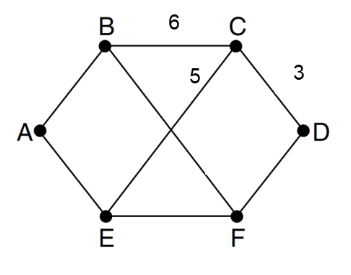
\includegraphics[width=0.5\linewidth]{distance-vector-diagram.png}
        \caption{Provided distance vector diagram}
    \end{figure}
}}


\begin{enumerate}
    \item What are the two most important network-layer functions in a computer network? What
    is the difference between them? (15 Points) \\ \answerOne
    \item Find all subnets in the following network. Write the IP address of those subnets in the
    subnet notation (i.e., a.b.c.d/x notation) (15 Points) \\\\ \answerTwo
    \item Consider the following network. With the indicated link costs, use Dijkstra’s shortest-path
    algorithm to compute the shortest path from x to all network nodes. Show how the
    algorithm works by computing a table similar to what we use in the lecture note. Also
    draw the resulting shortest-path tree from x to all nodes and the resulting forwarding
    table in x. (40 Points) \\\\ \answerThree    
    \item Consider the network of Figure. Distance vector routing is used, and the following vectors
    have just come in to router C: \\
    from B: (5, 0, 8, 3, 6, 2); \\
    from D: (6, 7, 6, 0, 9, 10); \\
    from E: (7, 6, 3, 2, 0, 4). \\
    The cost of the links from C to B, D, and E, are 6, 3, and 5, respectively. What is C’s new
    routing table? Give both the outgoing line to use and the cost. (30 Points) \\\\ \answerFour   
\end{enumerate}


\end{document}
